a\chapter{Implementation}
\label{sec:implementation}

% Hier greift man einige wenige, interessante Gesichtspunkte der
% Implementierung heraus. Das Kapitel darf nicht mit Dokumentation oder
% gar Programmkommentaren verwechselt werden. Es kann vorkommen, daß
% sehr viele Gesichtspunkte aufgegriffen werden müssen, ist aber nicht
% sehr häufig. Zweck dieses Kapitels ist einerseits, glaubhaft zu
% machen, daß man es bei der Arbeit nicht mit einem "Papiertiger"
% sondern einem real existierenden System zu tun hat. Es ist sicherlich
% auch ein sehr wichtiger Text für jemanden, der die Arbeit später
% fortsetzt. Der dritte Gesichtspunkt dabei ist, einem Leser einen etwas
% tieferen Einblick in die Technik zu geben, mit der man sich hier
% beschäftigt. Schöne Bespiele sind "War Stories", also Dinge mit denen
% man besonders zu kämpfen hatte, oder eine konkrete, beispielhafte
% Verfeinerung einer der in Kapitel 3 vorgestellten Ideen. Auch hier
% gilt, mehr als 20 Seiten liest keiner, aber das ist hierbei nicht so
% schlimm, weil man die Lektüre ja einfach abbrechen kann, ohne den
% Faden zu verlieren. Vollständige Quellprogramme haben in einer Arbeit
% nichts zu suchen, auch nicht im Anhang, sondern gehören auf Rechner,
% auf denen man sie sich ansehen kann.

% Implementation motivation

While chapter \ref{sec:design} presented the design of the developed
communication library, this chapter will pick up some design details
and focus on their implementation.  It is not intended to provide a
full documentation of the developed source code, moreover it should be
a guide in understanding the libarary. Therefore, documentation should
be retrieved from the source code or doxygen documentation
\cite{ref:doxygen}.

The library started from the need of PIConGPU (Section
\ref{sec:picongpu}) for a more flexibel and abstract communication
layer. PIConGPU is implemented in C++98 with additional usage of boost
\cite{ref:boost} libraries. Thus the communication library is also
implemented in C++. To make use of a richer feature set of the c++
language, C++11 is used \cite{ref:c++11}.

\section{The CAL with Policy Based Design}

The Communication Abstraction Layer was introduced in section
\ref{sec:cal} as a flexible Communication layer based on varying
adapters. The implementation of the varying adapters is based on
policy based design \cite{ref:policy_based_design}.

% Policy based design in general
A policy is a class or class template interface, which consists of
inner type definitions, member functions and/or member variables. An
implementation of a policy is called policy class and is inherited by
or contained within a host class.  The advantage of policy based
design is that the varying functionality of the policy is bounded to
its host class at compile time, providing no runtime overhead.  The
interface of the policy is strictly defined by the host
class. Ignoring this interface leads to errors at compile time.

% Policy based design for CAL + adapter
In the implementation of the CAL, the adapter is the policy, here
called communication policy, and the CAL is the host class (Figure
\ref{fig:cal_uml}). The CAL is configured by an adapter as template
argument and inheritates the adapter members in protected mode. The
CAL provides all communication and context operations discussed in
section \ref{sec:cal_context}. Adapter specific operations are
forwarded to the adapters interface, described in the following.

% CAL provides interface, adapter has to implement this interface

\begin{figure}[H]
  \centering 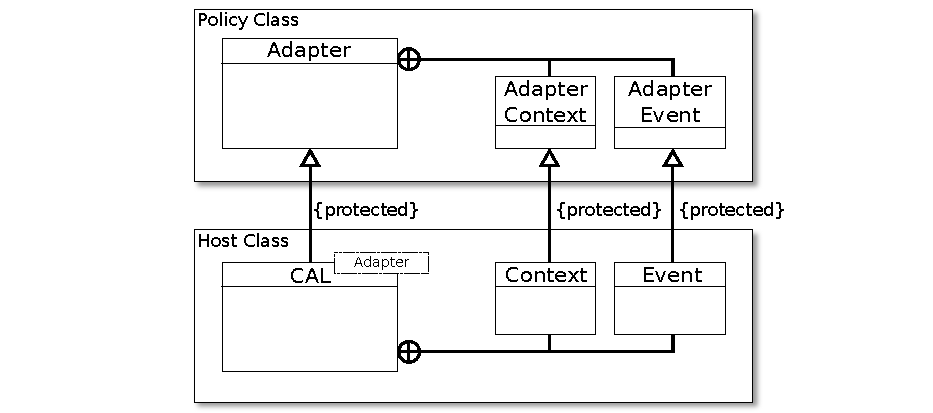
\includegraphics[width=\textwidth]{graphics/40_cal_uml}
  \caption{ }
  \label{fig:cal_uml}
\end{figure}

% Descrption Communication operations
Usually, the adapter has to provide all communication and context
operations the CAL defines. But, policy based design has the
characteristic that if a member function not used through the host
class, the compiler will not care if this function is not implemented
by the policy.  Thus only the used member functions have to be
implemented in an adapter (e.g. just peer to peer operations). But for
sake of completeness an adapter should implement the whole policy
interface.

% Description Context + Event
In addition to communication and context related member functions, the
adapter has also to provide a inner context and a inner event
class. Characteristics of these classes were explained in section
\ref{sec:cal_comm}. Both contain the adapter specific implementations,
thus, their implementation can not be discssed in detail. The
interface of these two inner adapter classes is defined by according
inner classes of the CAL. The functionality is implanted by
inheritance (Figure \ref{fig:cal_uml}).


\subsection{The MPI Adapter as Reference Implementation}
\label{sec:cal_mpi_adapter}
The reference adapter implementation is based on MPI as existing
communication layer.  MPI (Section \ref{sec:mpi}) was as choosen,
because it already provides a lot of functionality required by the CAL
interface from the scratch. Additionally it is available on wide range
of compute systems and can be used for free by open source
implementations. To address the message passing interface, the MPI C
language binding is used inside the adapter. An alternative would be
the boost::mpi C++ implementation, which presupposes that beside a MPI
implementation also the boost library is installed.

Implementing the communication operations is straight forward: in most
cases just a forwarding of arguments and a call of MPI C
functions. More tricky is the support of abitrary binary operations
for the reduce operation and the support of abitrary data types of the
exchanged data. Hence concepts to solve these two problems are
discussed.

\paragraph*{Binary Operator}

A collective reduce operation is based on an binary operator. The CAL
defined a very general binary operator in section
\ref{sec:cal_collective}. It can not be assumed that the general
binary operator is supported by every adapter, thus, it has to be
specialized to a binary operator the adapter can handle.


MPI has built-in support for binary operations, but they need to be
transformed by two possible approaches.  The simplest approach, is the
direct usage of binary MPI operators.  These can be defined in a
struct of static const expressions (Listing \ref{lst:mpi_bin}).
Hence, the CAL could forward the struct to the library user and the
user could select from these binary operations depending on the
reduction operation.

\begin{lstlisting}[language=C++, caption={A small collection of binary operators by transformed MPI operations to static constexpression }, label=lst:mpi_bin]
  struct BinaryOperations { static constexpr BinaryOperation MAX =
    MPI_MAX; static constexpr BinaryOperation MIN = MPI_MIN; static
    constexpr BinaryOperation SUM = MPI_SUM; static constexpr
    BinaryOperation PROD = MPI_PROD; };
\end{lstlisting}

The downside of the this approach is that only the predefined
operators of MPI can be used, restricting the application on this
limited set of operators Therfore, MPI gives the possibility to create
abitrary binary operators with the MPI\_Op\_create function, what can
be done for all binary operators. The source code for transforming
abitrary binary operators to binary MPI operators was taken over from
the boost::mpi project and adapted for the needs of the MPI adapter.
The only requirement of the CAL reduce interface, is that the binary
operation has to be like a struct discussed in section
\ref{sec:cal_collective}. This approach is essentially more flexible
then the first approach. Thus it was chooses to implement binary
operations for the MPI adapter.

\paragraph*{Data Type Conversion}

MPI predefines on one hand its primitive data types, but on the other
hand also provides the possibility to define own data structures based
upon sequences of the MPI primitive data types. Such user defined data
structures are called derived data types. Usually, Primitive data
types are contiguous. Derived data types allow you to specify
non-contiguous data in a convenient manner and to treat it as though
it was contiguous.  Thefore, more complex data types (e.g structs or
classes) have to be transformed into derived data types. The exchange
of complex data types was not necessary in the developement of library
based examples in section \ref{sec:gol_imp}, thus, the implementation
was focused on the transformation of primitive data types.  But
nevertheless, a transformation is available in the boost::mpi
implementation. Thus switching to boost::mpi \cite{ref:boost::mpi} or
adopting their source code would solve this problem without any
further effort.

The primitive C++ data types can be mapped directly to primitive MPI
data types. The conversation is implemented by the concept of traits
\cite{ref:trait}.  The function of the trait is the transformation of
primitive C++ data types to predefined MPI data types.  First, a
template struct defines the default behaviour of the trait (Listing
\ref{lst:mpi_trait1}). The struct defines a static const expression
with name type, which is set to a fixed MPI data type. The template
argument is the primitive data type that should be transformed. The
default struct will transform undefined data types to the MPI\_CHAR
data type.

\begin{lstlisting}[language=C++, label=lst:mpi_trait1]
  template<typename T> struct MPIDatatypes{ static constexpr
    MPI_Datatype type = MPI_CHAR; };
\end{lstlisting}

The following template is a explicit specialisation of the first
template, in this case for the C++ primitive data type int, which will
be transformed to the MPI\_INT data type (Listing
\ref{lst:mpi_trait2}). Thus, each transformation of a primitive C++
data type need to be defined.

\begin{lstlisting}[language=C++, label=lst:mpi_trait2]
  template<> struct MPIDatatypes<int>{ static constexpr MPI_Datatype
    type = MPI_INT; };

\end{lstlisting}

The communication operations within the adapter use the trait to
tranform the data types of the input and output data, by querying the
trait through MPIDataType<C++Datatype>::type.

\begin{itemize}
\item MPI specific Context \todo{MPI specific Context}
  

\item MPI specific Event

  Non-blocking communication operations return event objects.  MPI
  functions returns a request, which is the the event equivalent in
  the MPI world. A request is processed by MPI\_Wait to wait until the
  operation of the request has finished and MPI\_Test to check whether
  the operation has already finished.

\end{itemize}

\section{Graph Based on the Boost Graph Library}

BGL as backend The graph introduced in section \ref{sec:graph} was not
written from the scratch. There are a varity of libraries providing
graph implementations \todo{List some graph libaries}. Because of the
closeness of the boost library to the C++ STL, the boost graph library
\cite{ref:boost::bgl}, short BGL, was choosen. While the BGL provides
a lot of functionality, just a small subset is really needed for the
purposes of this work. Thus the BGL is wrapped inside a graph class
just providing standard graph funcionality.

\subsection{Vertices identified by Properties}

% Properties
Like in section \ref{sec:graph} discussed, a graph has so called
properties that can be used to describe its vertices and edges. The
BGL itself refers to vertices by integer numbers, whereby properties
of this integer vertices can be queried from so called property
maps. In this Graph, the vertices and edges are represented by its
property itself and are configured at compile time.  The properties
are structs or classes with abitrary content. However the properties
need to provide an id member variable to create an internal connection
of vertices to properties.  Thus asking for the vertices of the graph,
returns a vector of vertices. That vector is a list of vertex
properties in the context of the BGL, whereby every property is
connected by its id to the graph.

\subsection{Configuration of a Graph}
The configuration of the graph requires two classes to define both
vertex and edge property as template arguments.  If the graph should
not contain any further information then the properties will be filled
by default with a property only containing the id.

\subsection{Creation of a Graph}
A graph can be created by a list of edge descriptors and a list of
vertices, while an edge descriptor is tuple of source vertex,
destination vertex and the connecting edge. The vertices and edges can
allready be filled with property information.  This list of edge
descriptors can also generated by one of the several provided graph
generators. These allow a generation of commonly used graph
topologies.

\todo{explain graph generators?}

\subsection{Operations on the graph / vertices}
% Operations
The graph provides set of simple graph operations. Like retrieving all
vertices, retrieving adjacent vertices, retrieving in and out edges.
\todo{Is there more Information needed? Because it is not that
  interesting}

\subsection{Creation of subgraphs}
% Subgraph Createion
Another reason for the BGL is the builtin subgraph support. The
creation of subgraphs is meant to be used as an equivalent to the
creation of contexts in the CAL. Thus a subgraph can be created from
its supergraph by a subset of its vertices. Collective operations on
this subgraph only consider vertices within this subgraph.

\section{Graph-based Virtual Overlay network}

\begin{itemize}
\item Announce process

  The objective of the announcement process is the construction of a
  mapping from vertices of a graph to peers. In general, it is a
  collective operation of all the peers that want to take part on the
  communication of a specific graph.  These peers create first and
  foremost an exclusive context for themselves, which only contains
  peers that host verticesof the to announced graph.  Therfore the
  present most general context of these peers, possibly including more
  peers, has to be determined.  The overall most general context would
  be the global context of all peers in the network, but in some cases
  exists also a context with less peers. This is either the context of
  the graph or the context of the supergraph, if these graphs were
  allready announced.

  Afterwards a new context is created from the present one by
  gathering the number of vertices each peer hosts and every peer that
  hosts at least one vertex will belong to the new context.  Finally,
  The graph is mapped to the new context and will be used on further
  communication operations on this graph.

  The hosted vertices can now be distributed by a further gather
  operation in the new context and each peer updates its vertex map.

\item Communication

  Map vertices to peer adress.  Map graph to context.  Edge id is tag.
  Forward to CAL

\item Collective Operations locally

  Collective operations in the virtual overlay network are more
  complex than just forwarding the data to the CAL interface. Because
  peers host potentially more than one vertex, the collective
  operation has to be performed locally first.

  The implementation is a bit tricky because the data has an abitrary
  data type and a peer could mix the execution of collective
  operations of several graphs.

  Thus the data from hosted vertices of a peer is collected in a
  templated static vector until all hosted vertices of this peer have
  terminated their collective operation. Whereby, for every graph a
  new vector is created.

  When the last vertex terminates its collective operation, the
  operation is executed locally and then forwarded to the CAL
  interface. The CAL then executes the collective operation between
  all other peers of the graph.


\end{itemize}

\subsection{Configuration and Initialization of an Application}

Steps of Configuration

\begin{enumerate}
  % Configuration
\item Configure CAL
\item Configure graph with properties
\item Configure virtual overlay network with graph and CAL

  % Initialization
\item Create graph topologie
\item Create CAL object and retrieve intial context
\item Create virtual overlay network

  % Distribution and load balancing
\item Distribute vertices of graph to peers of context
\item Announce hosted vertices
\end{enumerate}

\section{Implementing a Game of Life}
\label{sec:gol_imp}
% Introduction
To show the communication library in a real world application, Game of
Life was implemented based on the developed communication library.

% GoL Graph based on Cells
The GoL world was modeled as a two-dimensional grid with diagonal
connections like the unbundled version in section \ref{sec:gol}. Thus
a GoL cell is represented by a vertex and neighboring cells are
connected by edges. The vertex property is set to the cell struct in
listing \ref{lst:gol_cell} and the edge property has no further
characteristics. The cell struct does contain the status information
of the cell and the id of the vertex, whereby 31.25 percent of all
cells are initialized with status alive.  The graph is generated by
the predefined graph generator for grids. The generator was configured
to create a two dimensional grid , while diagonal arranged cells are
connected (Figure \ref{fig:gol}).

\begin{lstlisting}[language=C++, label=lst:gol_cell]
  struct Cell { typedef unsigned ID; Cell() : id(0), isAlive(false){ }

    Cell(ID id) : id(id), isAlive(false){ unsigned random = rand() %
      10000; if(random < 3125){ isAlive = true; }

    }
    
    unsigned id; bool isAlive;

  };
\end{lstlisting}

% The CAL
The CAl is configured with the reference MPI adapter (Section
\ref{sec:cal_mpi_adapter}).  The graph vertices are then distributed
by the round robin method, which is by far no optimal vertex
distribution mehtod Other distribution methods are also possible
(Figure \ref{fig:gol_mapping}).


The distribution scales from one peer that gets all vertices to the
number of peers where every peer gets exactly one vertex. Distributing
the graph to more peers than available vertices is an interessting
case for fault tolerance and load balancing. Thus additional peers
could be used as backup peers. \todo{reference to ft and lb chapter}

Afterwards, every peer announces its hosted vertices on the virtual
overlay network. From this point on, starts the actual GoL algorithm.

\begin{figure}[H]
  \centering
  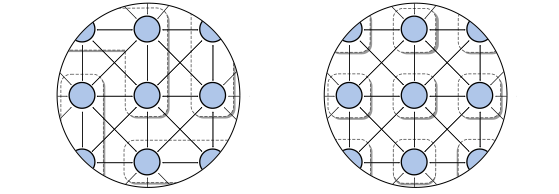
\includegraphics[width=\textwidth]{graphics/40_gol_mapping}
  \caption{Cut out of a GoL world. Abitrary distribution of
    displayed vertices to four available peers on the left
    side. While, on the right side, every peer hosts exactly one
    vertex.}
  \label{fig:gol_mapping}
\end{figure}

% The algorithm
In the following the implementation of a single evolution step of GoL
is described.  In the current situation, a peer has a list of vertices
it is responsible for. Thus, a peer has to manage the communication of
its vertices. In the case of GoL, a peer has to exchange the status of
its hosted cells and neihboring cells.

First, each peer has to send the status of its hosted cells to
neihboring cells . Therefore, the peer retrieves the target cells of
outgoing edges for a hosted cell from the graph . After that, the
status of the hosted cell is transmitted to the target cells
sequentially in non blocking mode (Figure
\ref{fig:gol_communication}). Events of the send operation are
collected and checked later for termination.

Second, each peer has to receive status information from neighboring
cells for each of its hosted cells. Therefore, the peer queries the
source cell of incoming edges for its hosted cells from the
graph. Further, it receives the status information from this
neighboring source cells.  The receive operation is used in blocking
mode, thus, all peers are synchronized afterwards.


\begin{figure}[H]
  \centering
  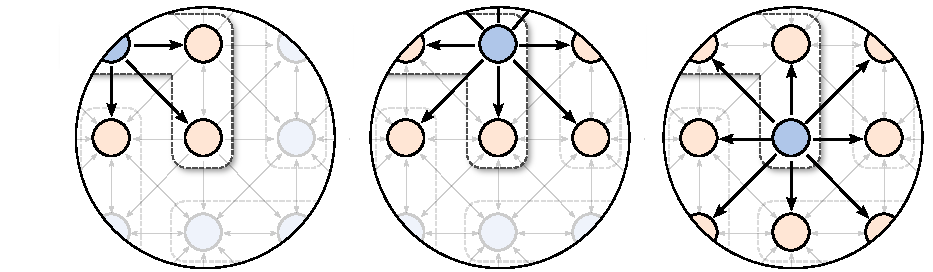
\includegraphics[width=\textwidth]{graphics/40_gol_communication}
  \caption{Cut out of a GoL world. A peer sends status information of
    hosted cells to neighboring cells. The communication operations
    are executed sequentially, but non blocking. Receive operations
    behave analog, but in blocking mode.}
  \label{fig:gol_communication}
\end{figure}


Once all send and receive operations have finished, the peer updates
the status of its hosted cells by the status of their neihboring
cells. Finally the status information of all cells is gathered by a
abitrary cell which prints it to the console for visualization and all
peers synchonize their program flow.  The next evolution steps will
repeat the previous steps until the application is aborted or a fixed
number of evolutions steps is reached.

% Modfifications
\begin{itemize}
\item Based on Bundles
\end{itemize}

\section{Redistribution of vertices}
\begin{itemize}
\item Vertices are not statically bounded to peers
\item Redistribution of vertices to a different peers is possible
\item Redistribution within a context of a graph is no problem
\item Redistribution to peers outside of context needs recreation of
  the context.

\item Load balancing in a vertex occupation scenario

  The communication library was always developed with the possibility
  of load balancing in mind.  Therefore, a occupation scenario was
  implemented to show a kind of load balancing at runtime.

  The scenario is the following: a peer occupies or steels a vertex
  from another peer and henceforward hosts this vertex.  This process
  is declared as occupation, because the change of the host is
  dictated by the so called master peer (Figure
  \ref{fig:gol_remapping}).

  \begin{figure}[H]
    \centering
    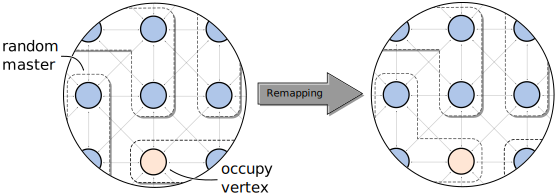
\includegraphics[width=\textwidth]{graphics/40_gol_remapping}
    \caption{Remapping of vertices to peers. A random master peer is
      determined by a consensus random number generation. The master
      dictates the vertex which will be occupied. Vertices of the
      graph are reannounced.}
    \label{fig:gol_remapping}
  \end{figure}

\item occupyRandomVertex - redistribution
  \begin{itemize}
  \item Swap of one vertex from one host to another
  \item determine random master
    
    Determining the master peer of a context is a randomized process
    by a collective operation. The master is the result of a random
    number modulo the size of the context. To find a consensus random
    number in the context, every peer generates an own random number
    and the consensus random number is calculated by accumulating all
    random numbers by a collective reduce operation.

  \item random master define vertex to occupy
    
    Once the master ist defined, it defines a occupy vertex of the
    graph. This vertex needs to be hosted from another peer of the
    graph, thus the master does not occupy a vertex from itself.
    
  \item broadcast occupy vertex to context

    The occupy vertex is broadcasted in the context and every peer in
    the context checks whether it hosts this occupy vertex. The peer
    hosting this vertex releases it, while the master adds the vertex
    to its hosted vertices.

  \end{itemize}
\item announce - reannounce
  \begin{itemize}
  \item Each peer retrieve updated list of hosted vertices

    Although, the peers know the master and the vertex that was
    occupied, distribution and announcement process are strictly
    seperated, thus the peers need to reannounce their hosted vertices
    of the graph. Even though nothing changed for the most peers.

  \item Announce again hosted vertices
  \end{itemize}


\end{itemize}


\cleardoublepage

%%% Local Variables:
%%% TeX-master: "diplom"
%%% End:
